%%%%%%%%%%%%%%%%%%%%%%%%%%%%%%%%%%%%%%%%%
% Beamer Presentation
% LaTeX Template
% Version 1.0 (10/11/12)
%
% This template has been downloaded from:
% http://www.LaTeXTemplates.com
%
% License:
% CC BY-NC-SA 3.0 (http://creativecommons.org/licenses/by-nc-sa/3.0/)
%
%%%%%%%%%%%%%%%%%%%%%%%%%%%%%%%%%%%%%%%%%

%----------------------------------------------------------------------------------------
%	PACKAGES AND THEMES
%----------------------------------------------------------------------------------------

%\pdfminorversion=4
\documentclass[10pt]{beamer}

\mode<presentation> {

% The Beamer class comes with a number of default slide themes
% which change the colors and layouts of slides. Below this is a list
% of all the themes, uncomment each in turn to see what they look like.

%\usetheme{default}
%\usetheme{AnnArbor}
%\usetheme{Antibes}
%\usetheme{Bergen}
%\usetheme{Berkeley}
%\usetheme{Berlin}
%\usetheme{Boadilla}
%\usetheme{CambridgeUS}
%\usetheme{Copenhagen}
%\usetheme{Darmstadt}
%\usetheme{Dresden}
%\usetheme{Frankfurt}
%\usetheme{Goettingen}
%\usetheme{Hannover}
%\usetheme{Ilmenau}
%\usetheme{JuanLesPins}
%\usetheme{Luebeck}
%\usetheme{Madrid}
%\usetheme{Malmoe}
%\usetheme{Marburg}
%\usetheme{Montpellier}
%\usetheme{PaloAlto}
%\usetheme{Pittsburgh}
%\usetheme{Rochester}
%\usetheme{Singapore}
%\usetheme{Szeged}
%\usetheme{Warsaw}


\usetheme[sectionpage=none]{metropolis} % https://github.com/matze/mtheme

% As well as themes, the Beamer class has a number of color themes
% for any slide theme. Uncomment each of these in turn to see how it
% changes the colors of your current slide theme.

%\usecolortheme{albatross}
%\usecolortheme{beaver}
%\usecolortheme{beetle}
%\usecolortheme{crane}
%\usecolortheme{dolphin}
%\usecolortheme{dove}
%\usecolortheme{fly}
%\usecolortheme{lily}
%\usecolortheme{orchid}
%\usecolortheme{rose}
%\usecolortheme{seagull}
%\usecolortheme{seahorse}
%\usecolortheme{whale}
%\usecolortheme{wolverine}

%\setbeamertemplate{footline} % To remove the footer line in all slides uncomment this line
%\setbeamertemplate{footline}[page number] % To replace the footer line in all slides with a simple slide count uncomment this line

%\setbeamertemplate{navigation symbols}{} % To remove the navigation symbols from the bottom of all slides uncomment this line
}


\usefonttheme{professionalfonts}
 % required for mathspec
\usepackage{mathspec}
%\setsansfont[BoldFont={Fira Sans},Numbers={OldStyle}]{Fira Sans Light}
\setsansfont[BoldFont={Fira Sans}]{Fira Sans Light}
\setmathsfont(Digits)[Numbers={Lining,Proportional}]{Fira Sans Light}



\usepackage{graphicx} % Allows including images
\usepackage{booktabs} % Allows the use of \toprule, \midrule and \bottomrule in tables
\usepackage{tikz}
\usepackage{tikz-3dplot}
\usepackage{tikz-dimline}
\usetikzlibrary{arrows.meta}
\usetikzlibrary{calc,angles,quotes} % angles, quotes = http://www.texample.net/tikz/examples/angles-quotes/
\usetikzlibrary{plotmarks} % https://tex.stackexchange.com/questions/140963/draw-a-filled-circle-at-every-point-of-a-tikz-plot#140967
%\usepackage{textpos}
\usepackage{pgf}
\usepackage{enumitem}

\usepackage{etoolbox} % For ifdef in footer
\usepackage[absolute, overlay]{textpos}

\usepackage{environ}
%%%%%%%%%%%%%%%%%%
% Code to scale a tikzpicture to textwidth (keeping correct font dimension).
% Preso da https://tex.stackexchange.com/questions/6388/how-to-scale-a-tikzpicture-to-textwidth#6391
% Necessita di \usepackage{environ} nel preambolo
% Usato cosi'
% \begin{scaletikzpicturetowidth}{\textwidth}
%   \begin{tikzpicture}[scale=\tikzscale]
%     \draw...
%   \end{tikzpicture}
% \end{scaletikzpicturetowidth}
%
\makeatletter
\newsavebox{\measure@tikzpicture}
\NewEnviron{scaletikzpicturetowidth}[1]{%
  \def\tikz@width{#1}%
  \def\tikzscale{1}\begin{lrbox}{\measure@tikzpicture}%
  \BODY
  \end{lrbox}%
  \pgfmathparse{#1/\wd\measure@tikzpicture}%
  \edef\tikzscale{\pgfmathresult}%
  \BODY
}
\makeatother














\DeclareGraphicsExtensions{.pdf, .png, .jpg} % Se due immagini hanno lo stesso nome sceglile secondo l'ordine di filetype qui
\graphicspath{ {./img/} }					 % Path delle immagini 





\newcommand{\nologo}{\setbeamertemplate{logo}{}}

% TODO use real file not test_
% FILE GENERATED AUTOMATICALLY

\newcommand{\myname}{Francesco Forcher}
\newcommand{\crystalname}{TCP76}
\newcommand{\runnumber}{5870}
\newcommand{\rundate}{2017-12-04}
\newcommand{\particletype}{Xenon}
\newcommand{\particleenergy}{95.6 GeV}

\newcommand{\xmin}{-0.875}
\newcommand{\xmax}{0.525}
\newcommand{\ymin}{-0.875}
\newcommand{\ymax}{0.525}

\newcommand{\torsionm}{1.8}
\newcommand{\torsionq}{-14.7}
\newcommand{\torsionmerr}{0.5}
\newcommand{\torsionqerr}{0.6}


%----------------------------------------------------------------------------------------
%	TITLE PAGE
%----------------------------------------------------------------------------------------

\title[Analysis of channeling for run \runnumber, crystal \crystalname.]
{Analysis of channeling for run \runnumber, crystal \crystalname} % The short title appears at the bottom of every slide, the full title is only on the title page
\subtitle{\textit{Run date: \rundate \\ Particle type: \particletype \\ Particle energy: \particleenergy} }


% \author{Francesco Forcher} % Your name
% \institute[UNIPD] % Your institution as it will appear on the bottom of every slide, may be shorthand to save space
% {
% Supervisors: \\ % Your institution for the title page
% M. Zanetti (UNIPD) \\
% D. Mirarchi (UNIPD) \\
% S. Redaelli (UNIPD) \\
% %\medskip
% %\textit{francesco.forcher@cern.ch} % Your email address
% }
\author{\textsc{\myname}} % Your name
\institute[UNIPD] % Your institution as it will appear on the bottom of every slide, may be shorthand to save space
{ }
\date{%
\textit{\today}
%\textit{Run date: 2017.05.16}\\
\vspace{1.5cm}} % Date, can be changed to a custom date

\logo{\begin{tikzpicture}[remember picture,overlay]%
\node[anchor=south west,yshift=1cm, xshift=0.95cm] at (current page.south west) {
\includegraphics[height=1cm]{img/CERN_LogoBadge.pdf}};
%\node[anchor=south west,yshift=1cm, xshift=2.5cm] at (current page.south west) {\includegraphics[height=1cm]{img/logoesigillo_unipd.pdf}};
%\node[anchor=east,yshift=-0.91cm, xshift=-1cm] at (current page.east) {\includegraphics[height=1.3cm]{img/logoesigillo_unipd.pdf}};
\node[anchor=south east,yshift=1cm, xshift=-0.85cm] at (current page.south east) {
\includegraphics[height=1cm]{img/be_dep_logo.pdf}};
\end{tikzpicture}}
% \logo{\begin{tikzpicture}[remember picture,overlay]%
% \node[anchor=south west,yshift=1cm, xshift=0.95cm] at (current page.south west) {\includegraphics[height=1cm]{img/logoesigillo_unipd.pdf}};
% \node[anchor=south west,yshift=1cm, xshift=4.5cm] at (current page.south west) {
\includegraphics[height=1cm]{img/CERN_LogoBadge.pdf}};
% %\node[anchor=east,yshift=-0.91cm, xshift=-1cm] at (current page.east) {\includegraphics[height=1.3cm]{img/logoesigillo_unipd.pdf}};
% \node[anchor=south east,yshift=1cm, xshift=-0.85cm] at (current page.south east) {
\includegraphics[height=1cm]{img/be_dep_logo.pdf}};
% \end{tikzpicture}}

\begin{document}


\addtobeamertemplate{frametitle}{}{%
\begin{tikzpicture}[remember picture,overlay]
\node[anchor=north east,yshift=5pt, xshift=5pt] at (current page.north east) {
\includegraphics[height=1cm]{img/CERN_LogoBadge_no_transparency.pdf}};
\end{tikzpicture}}




\begin{frame}
\titlepage % Print the title page as the first slide
\end{frame}

\nologo

% \begin{frame}
% \frametitle{Overview} % Table of contents slide, comment this block out to remove it
% \tableofcontents % Throughout your presentation, if you choose to use \section{} and \subsection{} commands, these will automatically be printed on this slide as an overview of your presentation
% \end{frame}

%----------------------------------------------------------------------------------------
%	PRESENTATION SLIDES
%----------------------------------------------------------------------------------------

\setbeamertemplate{frame footer}{\insertsection}
\metroset{titleformat section=smallcaps}
\metroset{titleformat frame=smallcaps}






%------------------------------------------------
\section{Geometrical cuts}
%------------------------------------------------
% 
% \begin{frame}
% \frametitle{Geometrical cuts}
% \begin{columns}[c] % The "c" option specifies centered vertical alignment while the "t" option is used for top vertical alignment
% 
% \column{.7\textwidth} % Left column and width
% \begin{figure}
% 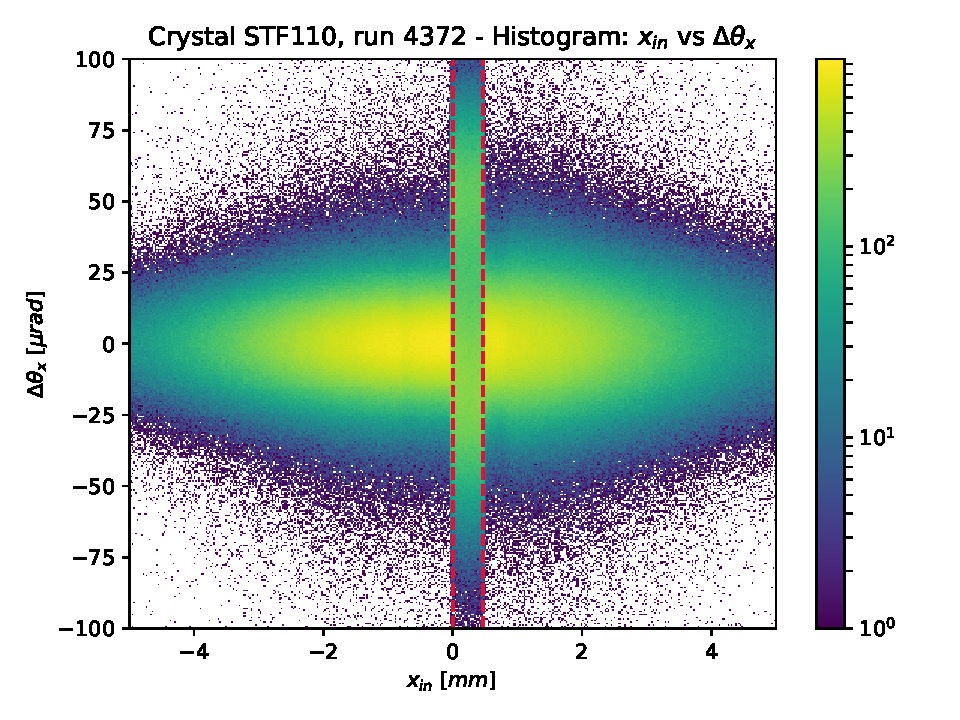
\includegraphics[width=\linewidth]{geocuts.pdf}\\
% %\caption{\footnotesize \itshape Istogramma delle deflessioni a seconda dell'angolo d'ingresso.}
% \end{figure}
% 
% \column{.3\textwidth} % Left column and width
% Istogramma delle deflessioni a seconda dell'angolo d'ingresso.
% 
% \end{columns}
% \end{frame}
% 

% \begin{frame}
% \frametitle{Geometrical cuts}
% 
% \begin{figure}
% 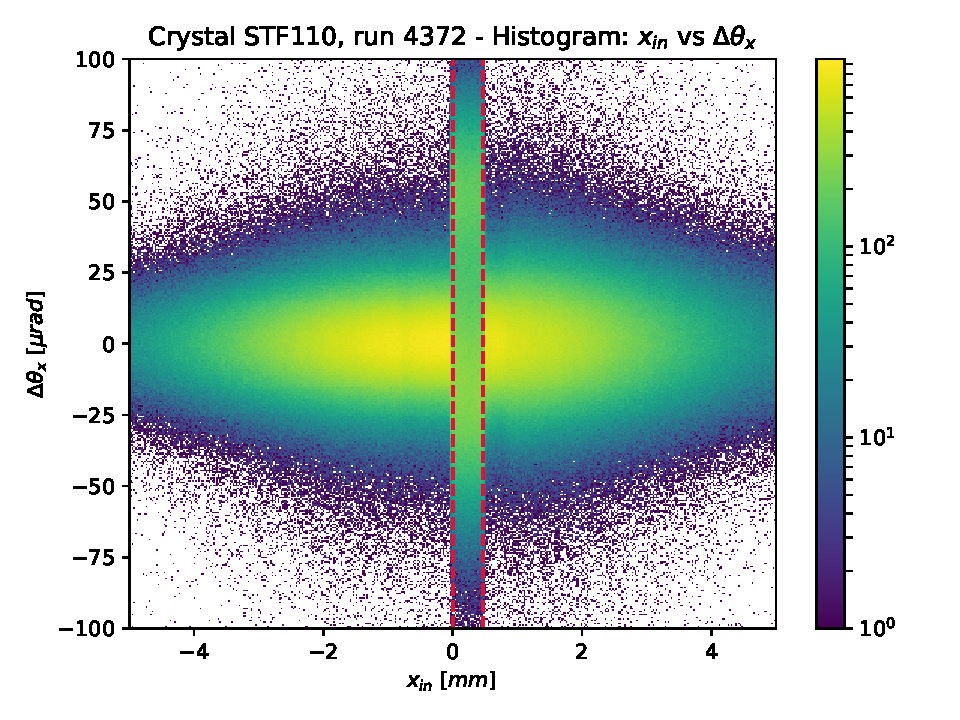
\includegraphics[width=0.8\linewidth]{geocuts.pdf}\\
% \caption{\footnotesize \itshape Geometrical cuts in x: \xmin\ -> \xmax\ [mm]}
% \end{figure}
% 
% \end{frame}
% 


\begin{frame}
\frametitle{Geometrical cuts}


\begin{columns}[c] % The "c" option specifies centered vertical alignment while the "t" option is used for top vertical alignment

\column{.7\textwidth} % Left column and width
\begin{figure}
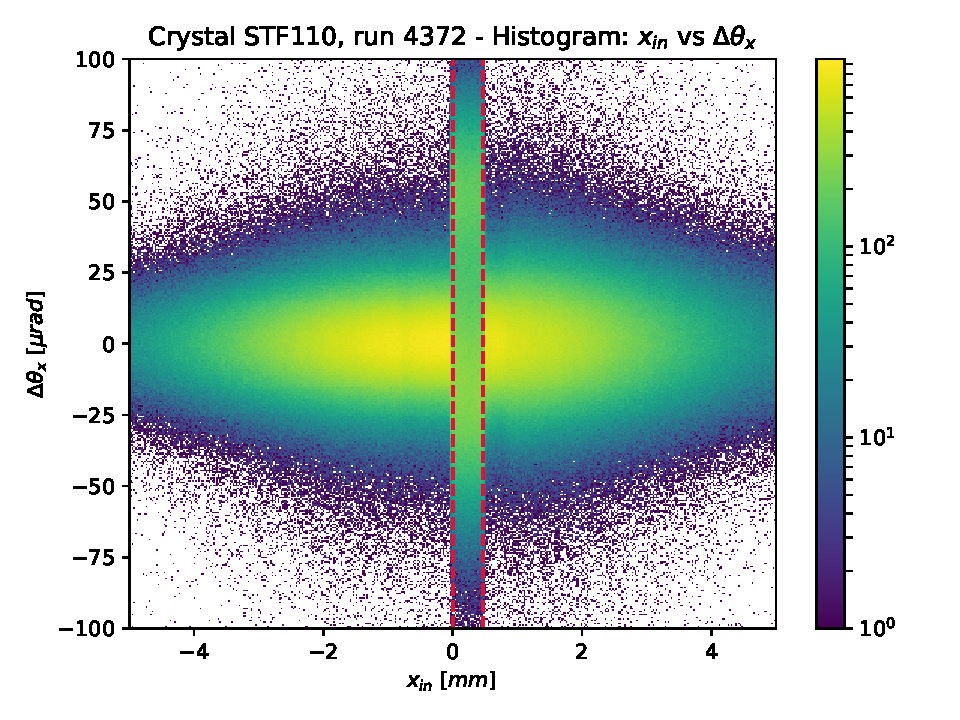
\includegraphics[width=\linewidth]{geocuts.pdf}\\
%\caption{\footnotesize \itshape Istogramma delle deflessioni a seconda dell'angolo d'ingresso.}
\end{figure}

\column{.3\textwidth} % Left column and width
Cuts in x:
\begin{itemize}[leftmargin=*]
 \item x1: \xmin\ [mm]
 \item x2: \xmax\ [mm]
\end{itemize}
Cuts in y:
\begin{itemize}[leftmargin=*]
 \item y1: \ymin\ [mm]
 \item y2: \ymax\ [mm]
\end{itemize}

\end{columns}
\end{frame}



%------------------------------------------------
\section{Torsion correction}
%------------------------------------------------


% 
% \begin{frame}
% \frametitle{Torsion analysis: efficiency}
% 
% \begin{figure}
% 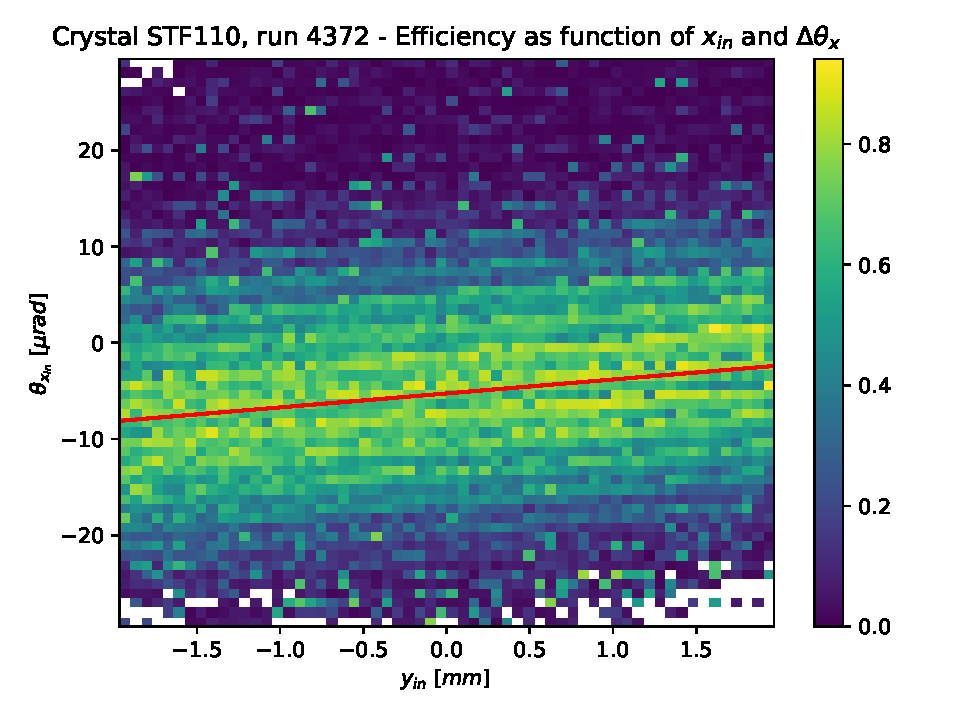
\includegraphics[width=0.8\linewidth]{efficiency_histo.pdf}\\
% %\caption{\footnotesize \itshape Efficiency plot: \xmin\ -> \xmax\ [mm]}
% \end{figure}
% 
% \end{frame}
% 



% \begin{frame}
% \frametitle{Torsion analysis: efficiency fit}
% 
% \begin{figure}
% 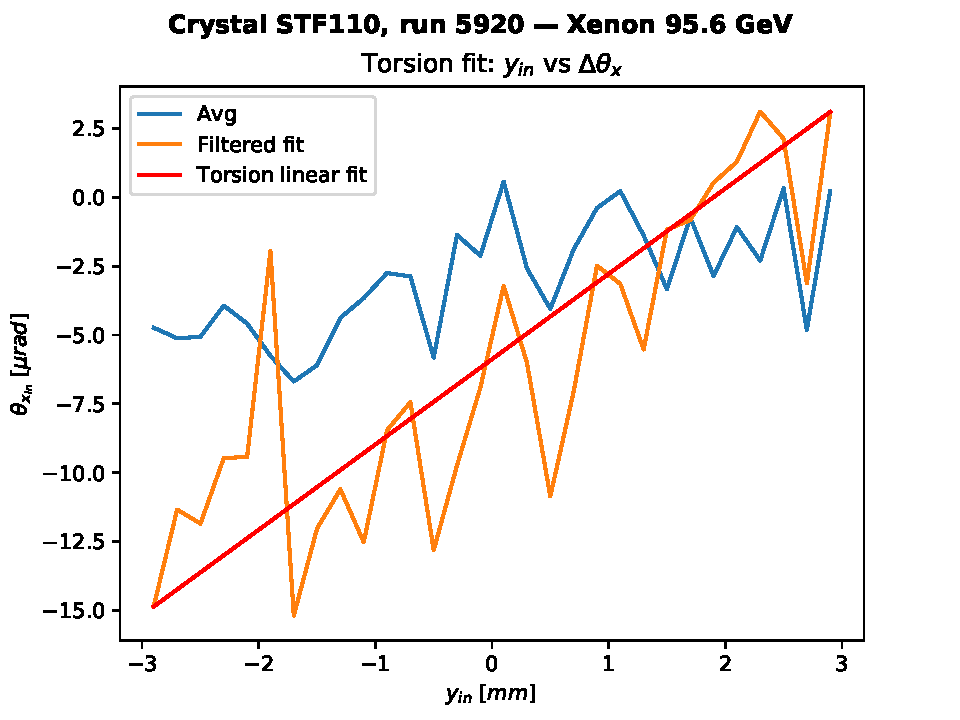
\includegraphics[width=0.8\linewidth]{torsion_fit.pdf}\\
% \caption{\footnotesize \itshape Efficiency fit: m: \torsionm\ [$\mu$rad / mm] --- q: \torsionq\ [$\mu$rad]}
% \end{figure}
% 
% \end{frame}





\begin{frame}
\frametitle{Torsion analysis: efficiency fit}
\vspace{-0.75cm}
\begin{columns}[t] % The "c" option specifies centered vertical alignment while the "t" option is used for top vertical alignment

\column{.6\textwidth} % Left column and width
\begin{figure}
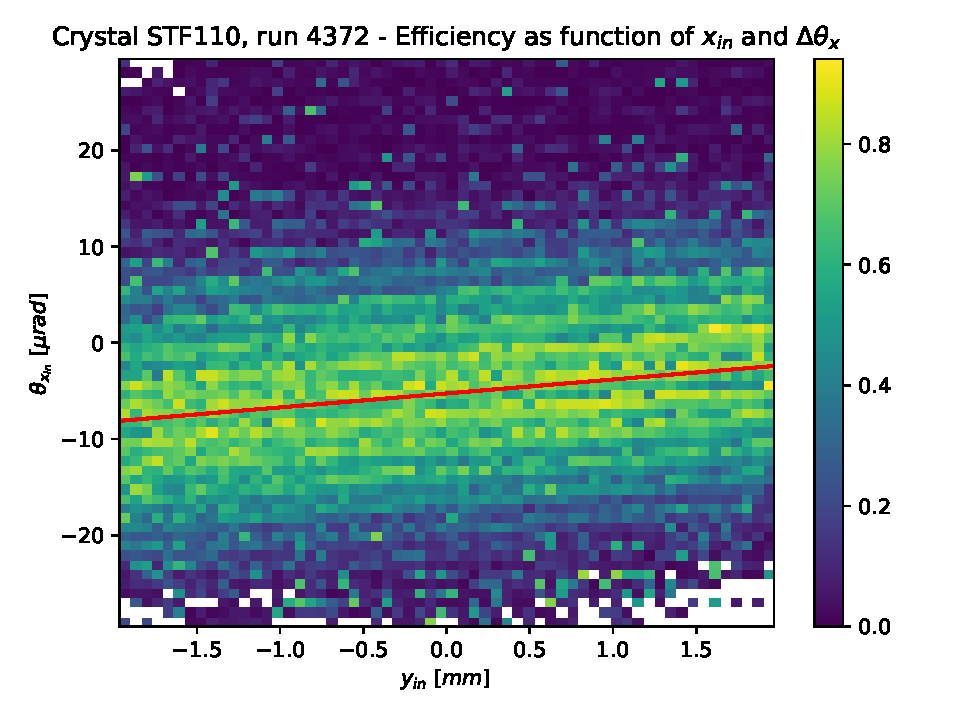
\includegraphics[width=\linewidth]{efficiency_histo.pdf}\\
%\caption{\footnotesize \itshape Istogramma delle deflessioni a seconda dell'angolo d'ingresso.}
\end{figure}

\column{.4\textwidth} % Left column and width
\begin{figure}
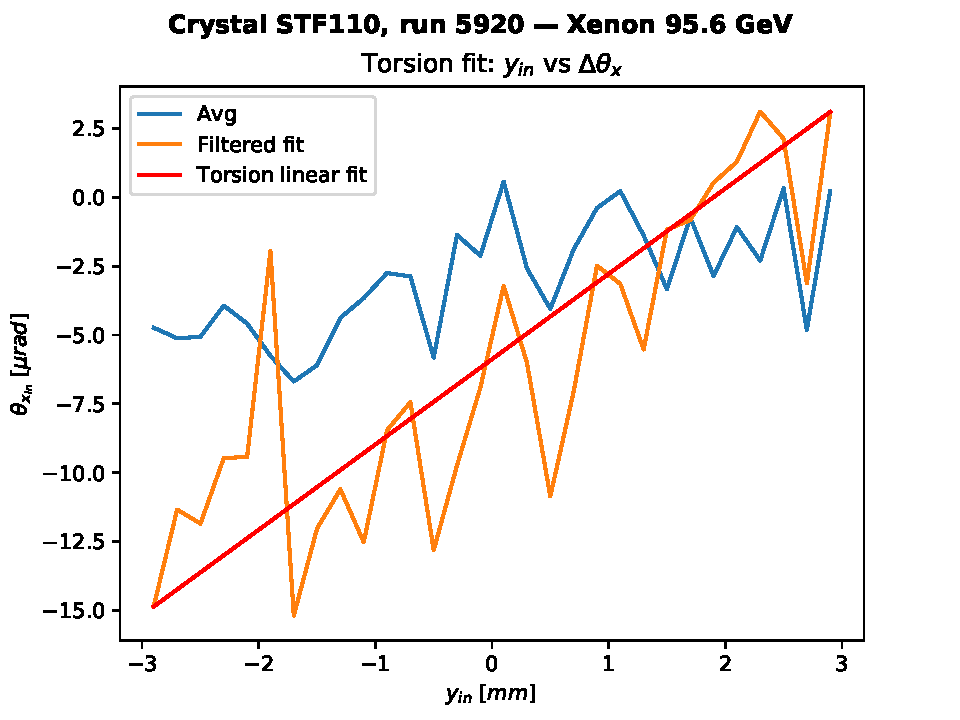
\includegraphics[width=\linewidth]{torsion_fit.pdf}\\
%\caption{\footnotesize \itshape Efficiency plot: \xmin\ -> \xmax\ [mm]}
\end{figure}

Efficiency fit:
\begin{itemize}[leftmargin=*]
 \item m: \torsionm\ [$\mu$rad/mm]
 \item q: \torsionq\ [$\mu$rad]
\end{itemize}


\end{columns}
\end{frame}


%------------------------------------------------
\section{Channeling analysis}
%------------------------------------------------

\begin{frame}
\frametitle{Deflection histograms}

\begin{columns}[c] % The "c" option specifies centered vertical alignment while the "t" option is used for top vertical alignment

\column{.5\textwidth} % Left column and width
\begin{figure}
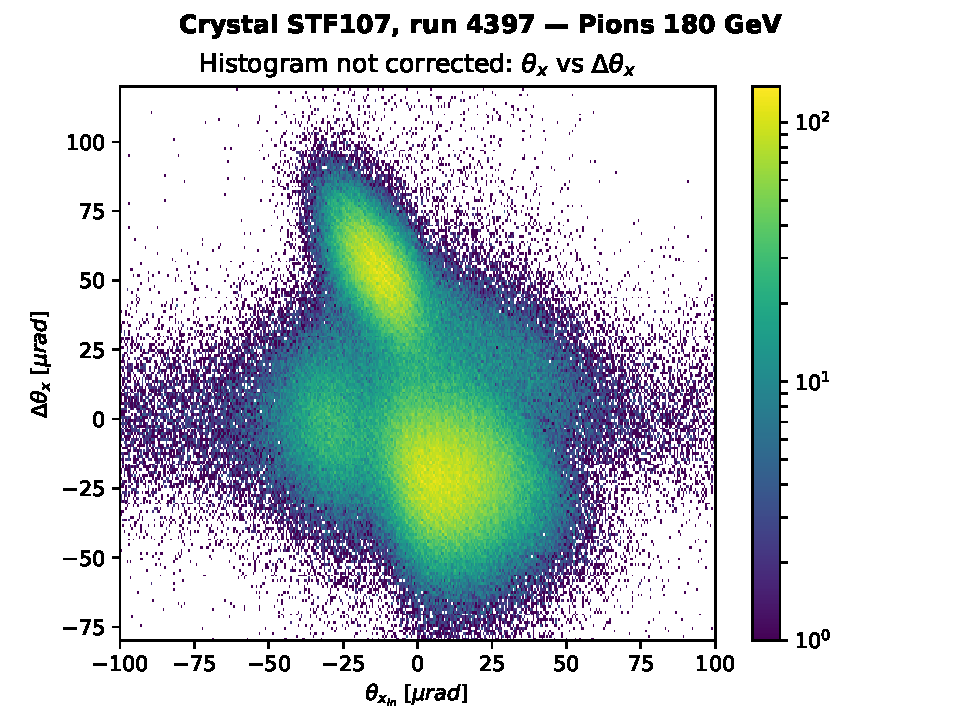
\includegraphics[width=0.9\linewidth]{nocorr_histo.pdf}\\
%\caption{\footnotesize \itshape Istogramma delle deflessioni a seconda dell'angolo d'ingresso.}
\end{figure}%
\vspace{-0.5cm}%
\begin{figure}
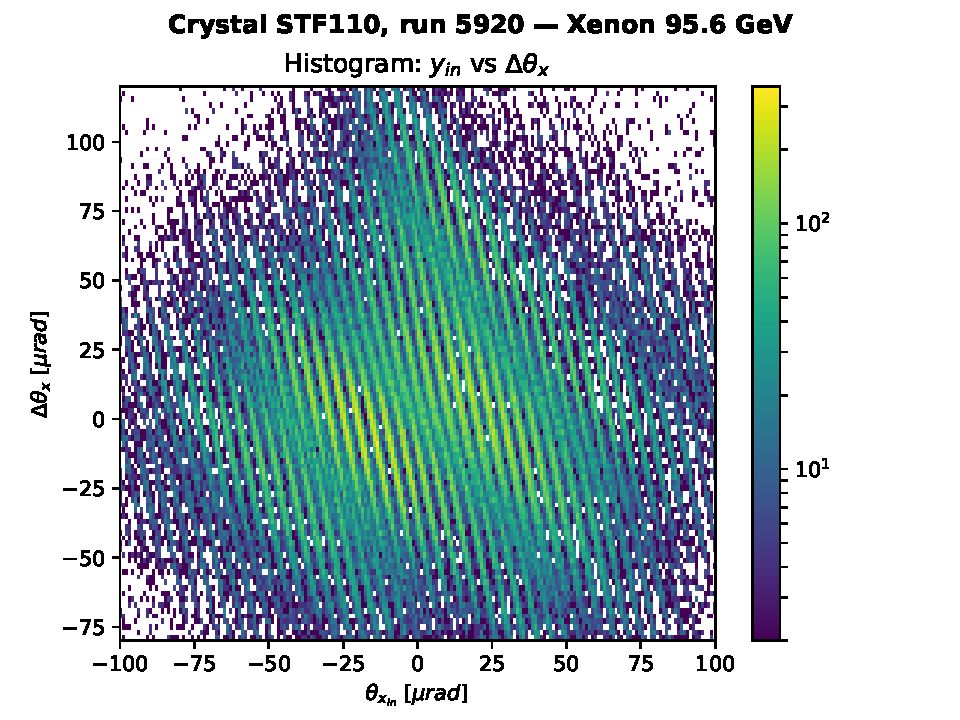
\includegraphics[width=0.9\linewidth]{corrected_histo.pdf}\\
%\caption{\footnotesize \itshape Istogramma delle deflessioni a seconda dell'angolo d'ingresso.}
\end{figure}

\column{.5\textwidth} % Left column and width
\begin{figure}
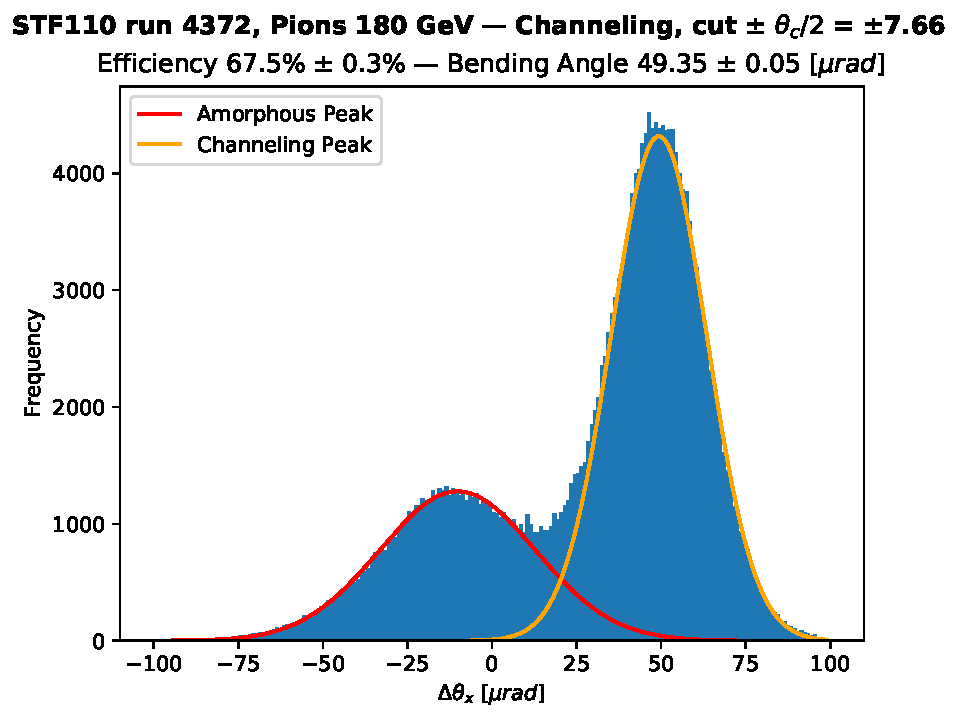
\includegraphics[width=0.9\linewidth]{half_thetac_chan_histo.pdf}\\
%\caption{\footnotesize \itshape Istogramma delle deflessioni a seconda dell'angolo d'ingresso.}
\end{figure}%
\vspace{-0.5cm}%
\begin{figure}
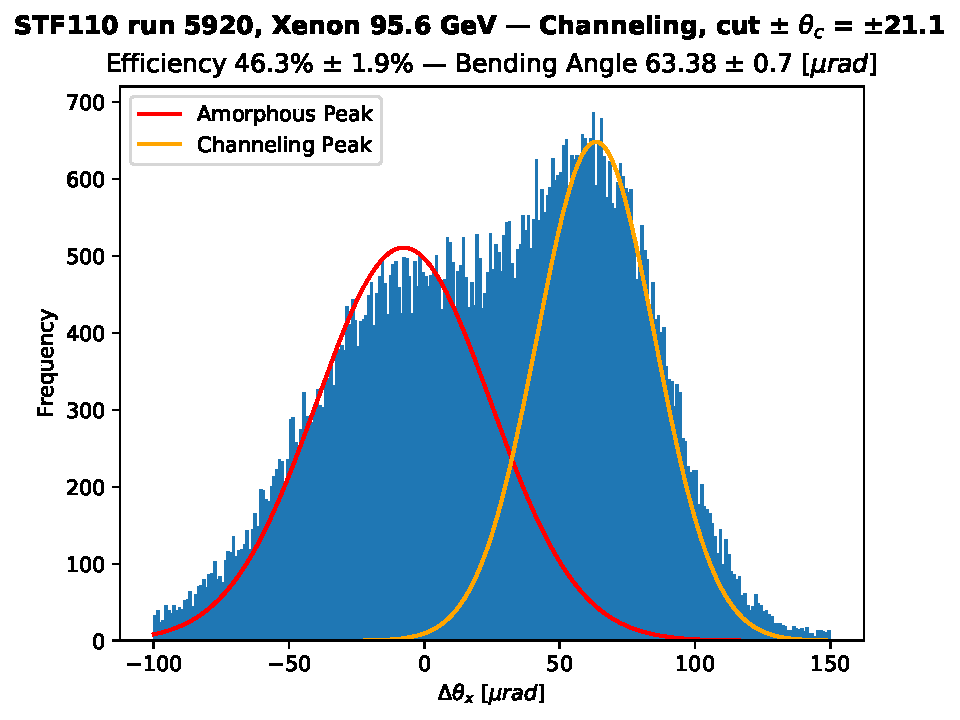
\includegraphics[width=0.9\linewidth]{thetac_chan_histo.pdf}\\
%\caption{\footnotesize \itshape Istogramma delle deflessioni a seconda dell'angolo d'ingresso.}
\end{figure}



\end{columns}
\end{frame}












% %------------------------------------------------
% \section{Channeling analysis}
% %------------------------------------------------

% \begin{frame}
% \frametitle{Channeling fit: cut at $\pm \frac{\theta_c}{2}$: half critical angle}
% 
% \begin{figure}
% 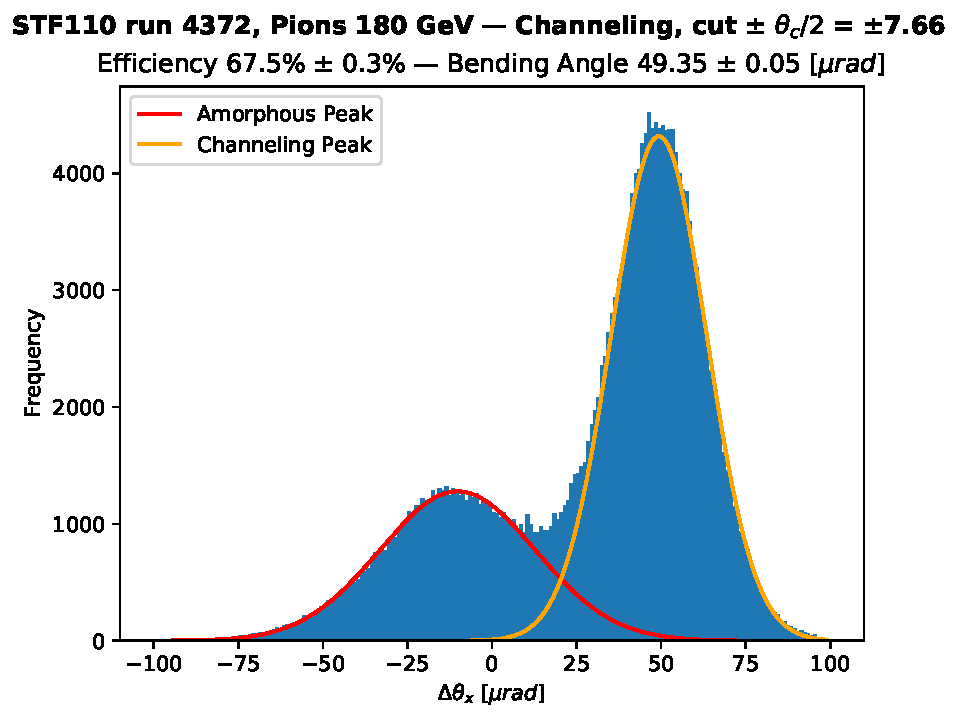
\includegraphics[width=0.8\linewidth]{half_thetac_chan_histo.pdf}\\
% %\caption{\footnotesize \itshape Efficiency plot: \xmin\ -> \xmax\ [mm]}
% \end{figure}
% 
% \end{frame}
% 
% 
% \begin{frame}
% \frametitle{Channeling fit: cut at $\pm \theta_c$: critical angle}
% 
% \begin{figure}
% 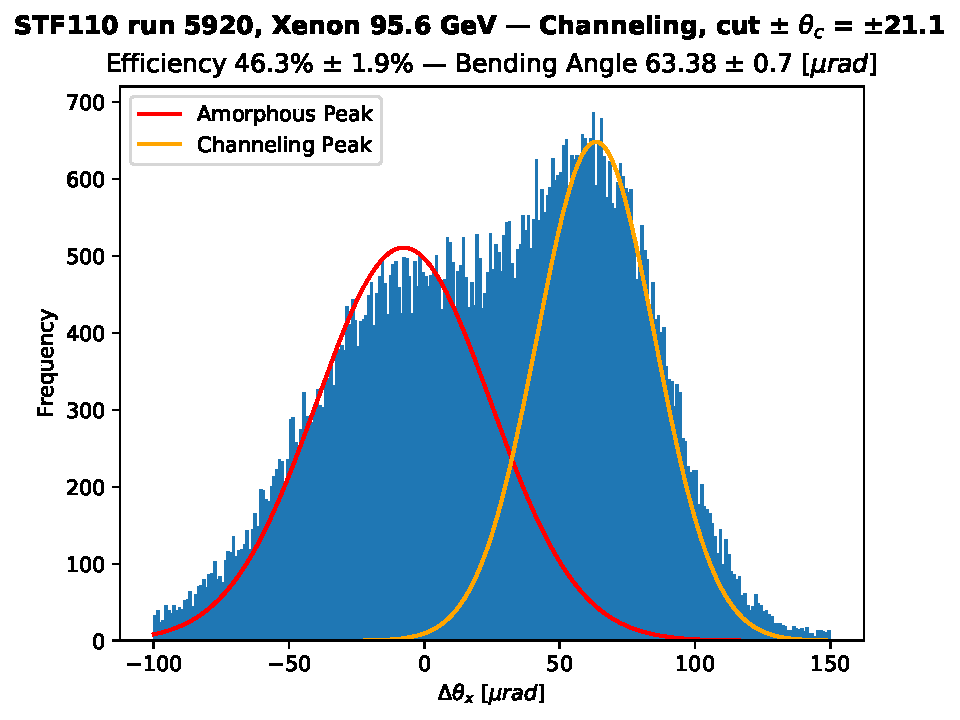
\includegraphics[width=0.8\linewidth]{thetac_chan_histo.pdf}\\
% %\caption{\footnotesize \itshape Efficiency plot: \xmin\ -> \xmax\ [mm]}
% \end{figure}
% 
% \end{frame}


% \begin{frame}
% \frametitle{Channeling fit: cuts at $\pm \frac{\theta_c}{2}$ and $\pm \theta_c$:}
% 
% \begin{columns}[c] % The "c" option specifies centered vertical alignment while the "t" option is used for top vertical alignment
% 
% \column{.5\textwidth} % Left column and width
% \begin{figure}
% 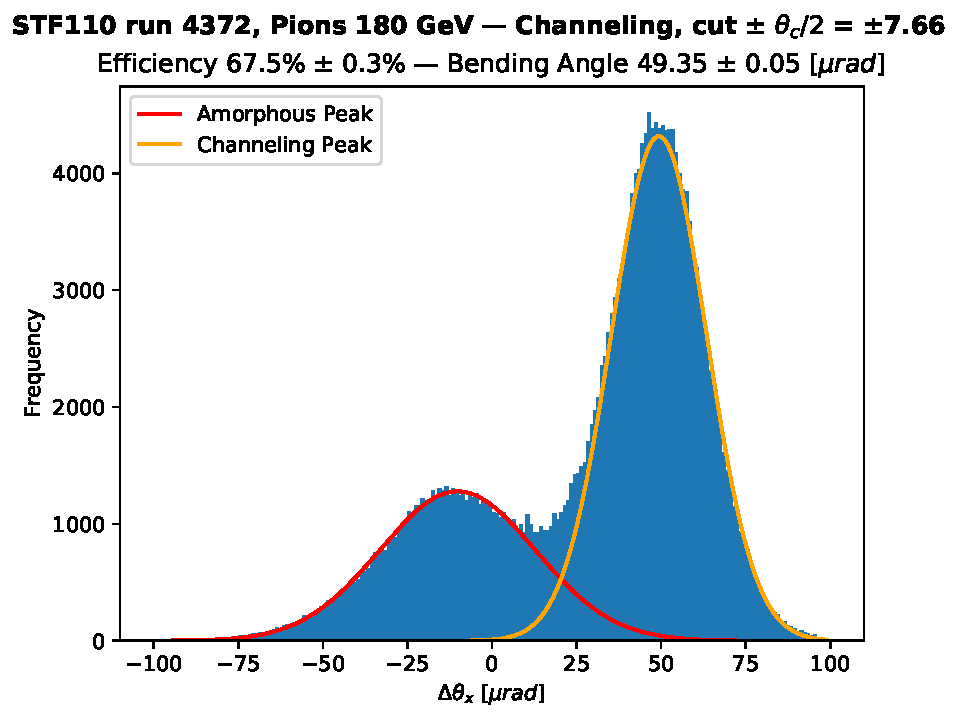
\includegraphics[width=\linewidth]{half_thetac_chan_histo.pdf}\\
% %\caption{\footnotesize \itshape Istogramma delle deflessioni a seconda dell'angolo d'ingresso.}
% \end{figure}
% 
% \column{.5\textwidth} % Left column and width
% \begin{figure}
% 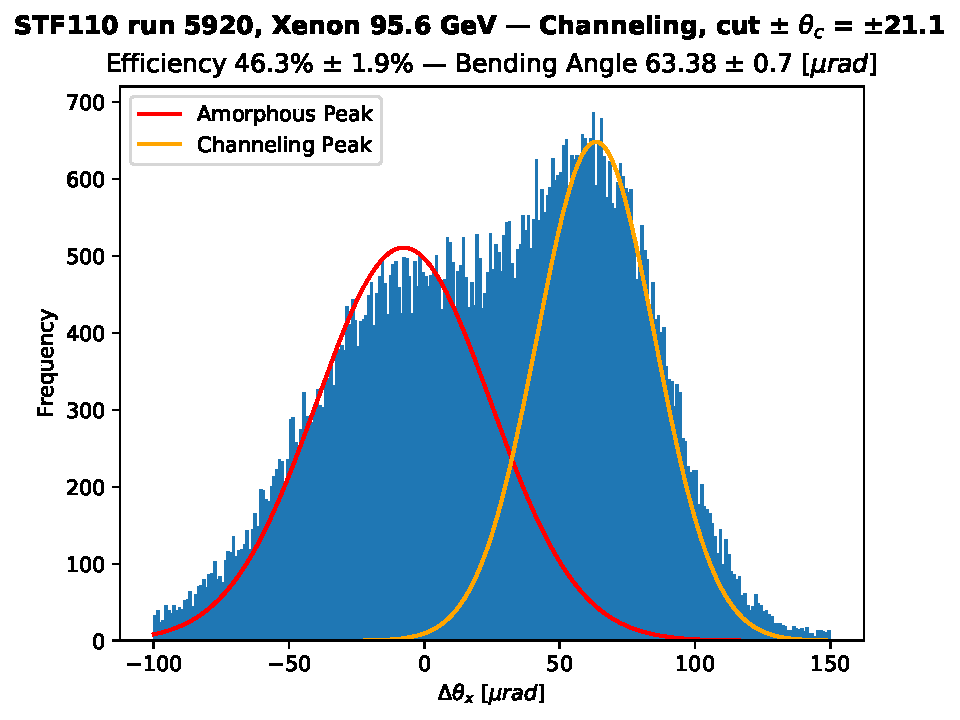
\includegraphics[width=\linewidth]{thetac_chan_histo.pdf}\\
% %\caption{\footnotesize \itshape Istogramma delle deflessioni a seconda dell'angolo d'ingresso.}
% \end{figure}
% 
% \end{columns}
% \end{frame}
% 
% 
% 

\end{document} 